{ % Command scope


\newcommand{\INSTANCE}{I}
\newcommand{\STORAGE}{S}
\newcommand{\PROVIDER}{P}
\newcommand{\PROVIDERINSTANCES}{PI}
\newcommand{\LOCALSTORAGE}{LS}

\newcommand{\LAYER}{L}
\newcommand{\TASK}{G}


\newcommand{\instancePrice}{p^I}
\newcommand{\ccu}{ccu}
\newcommand{\instanceTransferPriceIn}{p^{Iin}}
\newcommand{\instanceTransferPriceOut}{p^{Iout}}
\newcommand{\storageTransferPriceOut}{p^{Sout}}
\newcommand{\storageTransferPriceIn}{p^{Sin}}
\newcommand{\transferRate}{r}


\newcommand{\taskCount}{A^{tot}}
\newcommand{\transferTime}{t^{net}}
\newcommand{\execTime}{t^x}
\newcommand{\dataSizeIn}{d^{in}}
\newcommand{\dataSizeOut}{d^{out}}
\newcommand{\requestPrice}{p^{R}}
\newcommand{\workflowDeadline}{t^D}
\newcommand{\instanceDeadline}{t^d}
\newcommand{\unitTime}{t^u}
\newcommand{\transferCost}{c^T}
\newcommand{\tasksPerDeadline}{a^d}
\newcommand{\timeQuantum}{t^q}
\newcommand{\tasksPerTimeQuantum}{a^q}
\newcommand{\providerMaxMachines}{n^{Pmax}}
\newcommand{\instanceMaxMachines}{n^{Imax}}

\newcommand{\NumberInstances}{N}
\newcommand{\TaskAssignment}{A}
\newcommand{\DataAssignment}{D}
\newcommand{\TailTaskHours}{R}
\newcommand{\HasTail}{H}

\newcommand{\instanceSet}{I^{idx}}
\newcommand{\InstanceTasks}{T}
\newcommand{\InstanceHours}{H}
\newcommand{\InstanceActive}{A}
\newcommand{\LayerDeadline}{D}
\newcommand{\LayerTime}{D^t}

\chapter{Workflow optimization}
\label{chap:formulation-workflows} 
\lhead{Chapter \ref{chap:formulation-workflows}. \emph{Workflow optimization}}

    In this chapter we discuss optimization of scientific applications that may be represented as workflows. In Section \ref{sec:workflow:appmodel} we discuss the details of scietific workflows. Then in Section \ref{sec:workflow:problem} we formulate optimization problem using AMPL by defining the data, variables, constraints and the objective. Finally, in we evaluate in Section \ref{sec:workflow:evaluation} by scheduling example workflows from Workflow Generator Gallery.
  
    \section{Application model}
    \label{sec:workflow:appmodel}
    
    As described in Section \ref{intro:workflow}, a scientific workflow describes the dependencies between tasks and in most cases may be represented as directed acyclic graph (DAG), where nodes represent tasks and edges represent task dependencies. 
    
    There are different approaches to optimize workflow scheduling (see Chapter \ref{chap:state-of-art}). Mathematical programming allows to describe the model mathematically and use a set of available optimization solvers. On the other hand, an attempt to apply this method to the general problem of scheduling large-scale workflows on heterogeneous cloud resources would be impractical due to the problem complexity, therefore simplified models need to be analyzed. Optimization models can be simplified in several ways. We may simplify application model, infrastructure model or make certain assumptions on the schedule.
    
    In this model we assume that workflow is represented as a DAG. We also assume that a workflow is divided into several levels (layers) that can be executed sequentially and tasks within one level do not depend on each other (see Fig.~\ref{fig:workflow:appmodel}). Each layer represents a bag of tasks that can be partitioned in several groups (e.g. application A, application B, etc.) that share computational cost and input/output size. We assume that only one task group is executed on a specific cloud instance (VM). This forbids instance sharing between multiple layers, which means that each application needs its own specific VM template with a preconfigured environment.

    \begin{figure}[tb]
        \centering 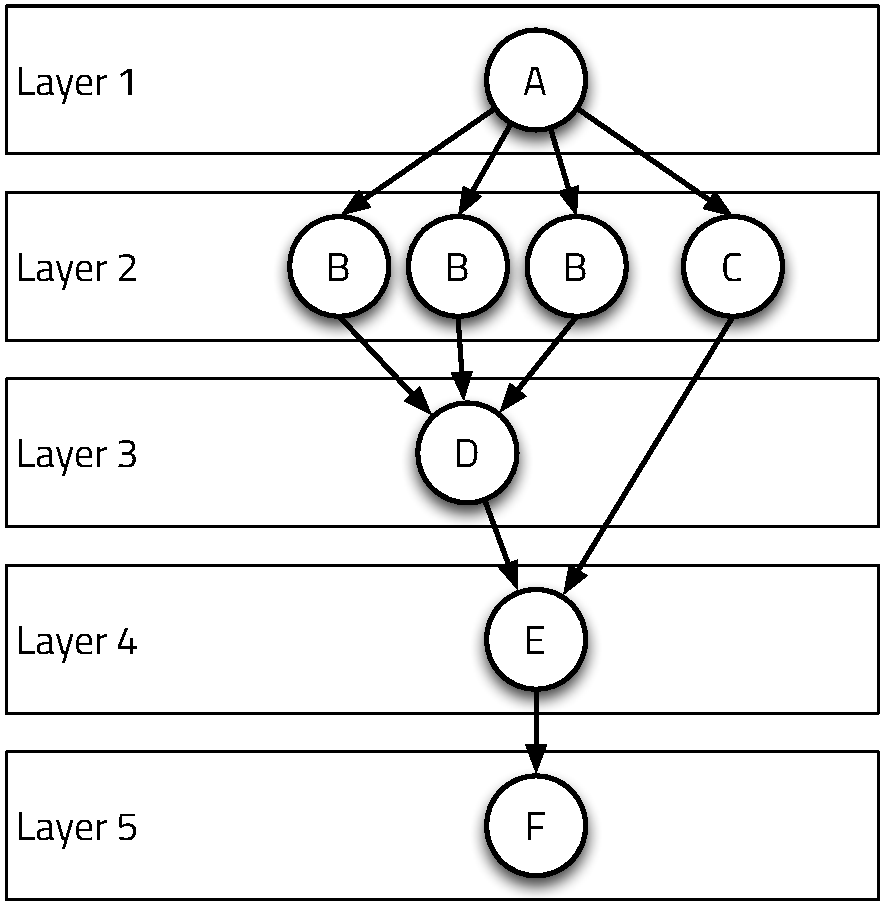
\includegraphics[width=0.5\columnwidth]{Workflow/workflow}
        \caption{Example application structure}
        \label{fig:workflow:appmodel}
    \end{figure}
    
    In this model we will use the same infrastructure model as presented in Section~\ref{sec:bot:cloudmodel}.
  
    \section{Problem formulation using AMPL}
    \label{sec:workflow:problem}
  
    Similarily to the model presented in Chapter~\ref{chap:bot} we will formulate and implement the model in AMPL.
    
    \subsection{Input data}
    \label{sec:workflow:problem:input}
     
    The formulation requires the following input sets, which represent the infrastructure model, in a similar way as we approached the problem in Chapter~\ref{chap:bot}:
    \begin{itemize}
        \item $\STORAGE = \{s3, cloudfiles\}$ -- defines available cloud storage
        sites,
        \item $\PROVIDER = \{amazon, rackspace, \dotsc\}$ -- defines
        possible computing cloud providers,
        \item $\INSTANCE = \{m1.small, \dots, gg.1gb, \dotsc\}$ -- defines
        instance types,
        \item $\PROVIDERINSTANCES_{p} \subset \INSTANCE$ -- instances that
        belong to provider $\PROVIDER_p$,
        \item $\LOCALSTORAGE_{s} \subset \PROVIDER$ -- compute cloud providers
        that are local to storage platform $\STORAGE_s$.
    \end{itemize}        
        
    Each instance type $\INSTANCE_i$ is described by the following parameters:
    \begin{itemize}
        \item $\instancePrice_i$ -- fee in \$ for running instance $\INSTANCE_i$
        for one hour,
        \item $\ccu_i$ -- performance of instance in CloudHarmony Compute Units
        (CCU),
        \item $\instanceTransferPriceOut_i$ and $\instanceTransferPriceIn_i$ --
        price for non-local data transfer to and from the instance, in \$ per
        MiB (1 MiB = $1024*1024$ Bytes)
    \end{itemize}
    
    Storage sites are characterized by:
    \begin{itemize}
        \item $\storageTransferPriceOut_s$ and $\storageTransferPriceIn_s$
        characterize price in \$ per MiB for non local data transfer.
    \end{itemize}
    
    Additionally we need to provide data transfer rates in MiB per second between
    storage and instances by defining function $\transferRate_{i,s} > 0$ .
    
  
    Our application model is different from the one in~Chapter~\ref{chap:bot} because it groups tasks into layers:

    \begin{itemize}
        \item $\LAYER$  -- set of layers,
        \item $\TASK$   -- set of tasks groups,
        \item $\TASK_l$ -- set of tasks groups belonging to layer $l$, 
        \item $\taskCount_t$ -- number of tasks in group $t$,
        \item $\execTime_t$ -- execution time in hours of a single task of group $t$ on 1 CCU
        machine,
        \item $\dataSizeIn_t$ and $\dataSizeOut_t$ -- data size for input and
        output of one task $t$ in MiB,
        \item $\requestPrice$ -- price per request for queuing service, such as Amazon SQS, required to execute a single task,
        \item $\workflowDeadline$ -- total time for completing workflow (deadline).
    \end{itemize} 
    
    \subsection{Auxiliary parameters}
    \label{sec:workflow:problem:auxiliary}
    
    A set of precomputed parameters which are derived from the main input parameters of the model includes:
     \begin{align}
         \transferTime_{i,s} &= \frac{\dataSizeIn+\dataSizeOut}{\transferRate_{i,s} \cdot 3600}  \\
         \label{workflow:unitTime}\unitTime_{i,s} &= \frac{\execTime}{\ccu_i} + \transferTime_{i,s}  \\
         \begin{split}
             \transferCost_{i,s} &= (\dataSizeOut \cdot
             (\instanceTransferPriceOut_i + \storageTransferPriceIn_s) \\ & +
             \dataSizeIn \cdot (\storageTransferPriceOut_s+\instanceTransferPriceIn_i)) \end{split} \\
     \end{align}
    \begin{itemize}
        \item $\transferTime_{i,s}$ -- {\em transfer time}: time for data transfer between
        $\INSTANCE_i$ and $\STORAGE_s$,
        \item $\unitTime_{i,s}$ -- {\em unit time}: time for processing a task
        on instance $\INSTANCE_i$ using storage $\STORAGE_s$ that includes computing and
        data transfer time (in hours),
        \item $\transferCost_{i,s}$ -- cost of data transfer between instance
        $\INSTANCE_i$ and storage $\STORAGE_s$,
        \item $\instanceSet_i$ -- set of possible instance $\INSTANCE_i$ indexes (from $0$ to $\instanceMaxMachines_i - 1$).
    \end{itemize}
   
    \subsection{Variables}
    \label{sec:workflow:problem:variables}
    Variables that will be optimized and define the solution space are:
    \begin{itemize}
        \item $\InstanceActive_{t,i,x}$ -- binary, $1$ iif (if and only if) instance $\INSTANCE_i$ with index $x$ is launched to process task group $\TASK_t$, otherwise $0$;
        \item $\InstanceHours_{t,i,x}$ -- integer, for how many hours is instance launched;
        \item $\InstanceTasks_{t,i,x}$ -- integer, how many tasks of $\TASK_t$ are processed on that instance,
        \item $\LayerTime_l$ -- actual computation time for $\LAYER_l$,
        \item $\LayerDeadline_l$ -- integer, maximal number of hours that instances are allowed to run in $\LAYER_l$.
    \end{itemize}
    
    \subsection{Formulation of objectives}
    \label{sec:workflow:problem:objective}
    
    Cost of running one task including instance and transfer cost is:

    \begin{align}
        \left(\transferTime + \unitTime\right) \cdot \instancePrice + 
        \dataSizeIn \cdot \left(\storageTransferPriceOut + \instanceTransferPriceIn\right) + 
        \dataSizeOut \cdot \left(\instanceTransferPriceOut + \storageTransferPriceIn\right) + 
        \requestPrice
    \end{align}

    while the objective function represents the total cost of running multiple
    tasks of the application on the cloud infrastructure is defined as:
    
    \begin{align}    
    \begin{split}
        \underset{\text{total cost}}{\text{minimize}} \sum \limits_{t \in \TASK, i \in \INSTANCE, x \in \instanceSet_i}  ( & 
                    (\instancePrice_i * \InstanceHours_{t,i,x} + \requestPrice + \transferCost_{i,s})*\InstanceTasks_{t,i,x} 
                   )
    \end{split}
    \end{align}
      
   subject to the constraints:
   \nopagebreak 
   \begin{align}
       \label{workflow:cLayerDeadline} \mathop\sum\limits_{l \in \LAYER} & \LayerDeadline_l \leq \workflowDeadline
       \\
       \label{workflow:cLayerTime}     \mathop\forall\limits_{l \in \LAYER} & \LayerTime_l \leq \LayerDeadline_l \leq \LayerTime_l + 1
       \\
       \label{workflow:cInstancesActiveHours} \mathop\forall\limits_{t \in \TASK, i \in \INSTANCE, x \in \instanceSet_i} & 
         \InstanceActive_{t,i,x} \leq \InstanceHours_{t,i,x} \leq  \InstanceActive_{t,i,x} \cdot \workflowDeadline
       \\
       \label{workflow:cInstancesActiveTasks} \mathop\forall\limits_{t \in \TASK, i \in \INSTANCE, x \in \instanceSet_i} &
         \InstanceActive_{t,i,x} \leq \InstanceTasks_{t,i,x} \InstanceActive_{t,i,x} \cdot \taskCount_t
       \\
       \label{workflow:cEnsureLayerDeadline} \mathop\forall\limits_{t \in \TASK, i \in \INSTANCE, x \in \instanceSet_i} &
         \InstanceHours_{t,i,x} \leq \LayerDeadline_l
       \\ 
       \label{workflow:cEnsureLayerTime} \mathop\forall\limits_{l \in \LAYER, t \in \TASK_l, i \in \INSTANCE, x \in \instanceSet_i} &
         \InstanceTasks_{t,i,x} \cdot \unitTime_{t,i,s} \leq \LayerTime_l
       \\       
       \label{workflow:cEnoughProcessingPower} \mathop\forall\limits_{t \in \TASK, i \in \INSTANCE, x \in \instanceSet_i} &
         \InstanceTasks_{t,i,x} \cdot \unitTime_{t,i,s} \leq \InstanceHours_{t,i,x} \InstanceTasks_{t,i,x} \cdot \unitTime_{t,i,s} + 1\\
       \\         
       \label{workflow:cProcessAllTasks} \mathop\forall\limits_{t \in \TASK} &
         \mathop\sum\limits_{i \in \INSTANCE, x \in \instanceSet_i} \InstanceTasks_{t,i,x} = \taskCount_t
       \\
       \label{workflow:cSymmetricSolutions1} \mathop\forall\limits_{t \in \TASK, i \in \INSTANCE, x \in \left\{1 .. \left(\instanceMaxMachines_i - 1\right)\right\}} & 
         \InstanceHours_{t,i,x} \leq \InstanceHours_{t,i,x-1} \\        
       \label{workflow:cSymmetricSolutions2} \mathop\forall\limits_{t \in \TASK, i \in \INSTANCE, x \in \left\{1 .. \left(\instanceMaxMachines_i - 1\right)\right\}} & 
         \InstanceActive_{t,i,x} \leq \InstanceActive_{t,i,x-1}\\ 
       \label{workflow:cSymmetricSolutions3} \mathop\forall\limits_{t \in \TASK, i \in \INSTANCE, x \in \left\{1 .. \left(\instanceMaxMachines_i - 1\right)\right\}} &
         \InstanceTasks_{t,i,x} \leq \InstanceTasks_{t,i,x-1}
       \\
       \label{workflow:cProviderLimits} \mathop\forall\limits_{l \in \LAYER, p \in \PROVIDER} &
         \mathop\sum\limits_{i \in \PROVIDERINSTANCES_p, t \in \TASK_l, x \in \instanceSet_i} \InstanceActive_{t,i,x} \leq \providerMaxMachines_p
    \end{align}
    
    Interpretation of the constraints is the following:
    \begin{itemize}
        \item(\ref{workflow:cLayerDeadline}) ensures that workflow finishes in given deadline,
        \item(\ref{workflow:cLayerTime}) fix that $\LayerDeadline = \ceil{\LayerTime}$,
        \item(\ref{workflow:cInstancesActiveHours}) ensure that $\InstanceHours$ may be allocated only iif $\InstanceActive$ is $1$,
        \item(\ref{workflow:cInstancesActiveTasks}) ensure that $\InstanceTasks$ may be allocated only iif $\InstanceActive$ is $1$,
        \item(\ref{workflow:cEnsureLayerDeadline}) enforces layer deadline on instances runtime,
        \item(\ref{workflow:cEnsureLayerTime}) enforces layer finishes work in $\LayerTime$,
        \item(\ref{workflow:cEnoughProcessingPower}) adjust $\InstanceHours$ respectively to $\InstanceTasks$ in order to make sure that all the instances run for enough time to process all tasks allocated to them we require,
        \item(\ref{workflow:cProcessAllTasks}) ensures that all tasks are processed,
        \item(\ref{workflow:cSymmetricSolutions1} to \ref{workflow:cSymmetricSolutions3}) reject symmetric solutions,
        \item(\ref{workflow:cProviderLimits}) enforces instance limits per cloud.
    \end{itemize}
    
    To keep this model in MIP class we had to take different approach than in previous model, and schedule each virtual machine instance separately. The drawback of this approach is that we need to increase the number of decision variables. The search space is also divided by storage provider. Additionally, the deadline becomes a variable with upper bound as it may happen that shorter deadline may actually give a cheaper solution (see Fig.~\ref{fig:workflow:genome-500-ratio} and its discussion).
    
    
    \section{Evaluation}
    \label{sec:workflow:evaluation}

    To evaluate our model on realistic data, we use CloudHarmony~\cite{CloudHarmony} benchmarks to parameterize the infrastructure model, and we use the Workflow  Generator Gallery workflows~\cite{Bharathi08} as test applications.

    In the infrastructure model we assumed that we have 4 public cloud providers (Amazon EC2, RackSpace, GoGrid and ElasticHosts) and a private cloud with 0 cost. The infrastructure has two object storage services, S3 that is local to EC2 and CloudFiles that is local to RackSpace, so data transfers between local compute and storage are free. 

    We tested our model with all application types from the gallery: Montage, CyberShake, Epigenomics, LIGO and SIPHT for all available workflow sizes (from 50 to 1000 tasks per workflows, up to 5000 tasks in the case of SIPHT workflow). We varied the deadline from 1 to 30 hours with 1-hour increment. We solve the problem for two cases, depending on whether the data is stored on Amazon S3 or on RackSpace CloudFiles.
  
    \begin{figure}[b] 
       \centering
       \begin{subfigure}[b]{0.49\textwidth}  
         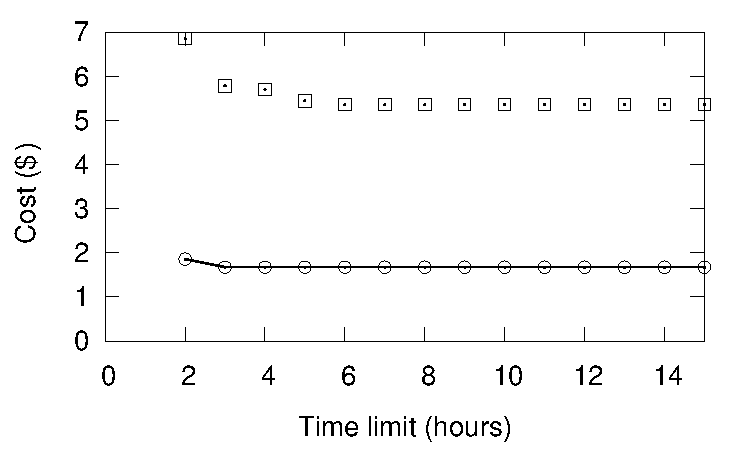
\includegraphics[width=\textwidth]{Workflow/Genome400-deadline_cost}
         \caption{400 tasks, 1 GiB data size}
         \label{fig:workflow:genome-400}
       \end{subfigure}
       \begin{subfigure}[b]{0.49\textwidth}
         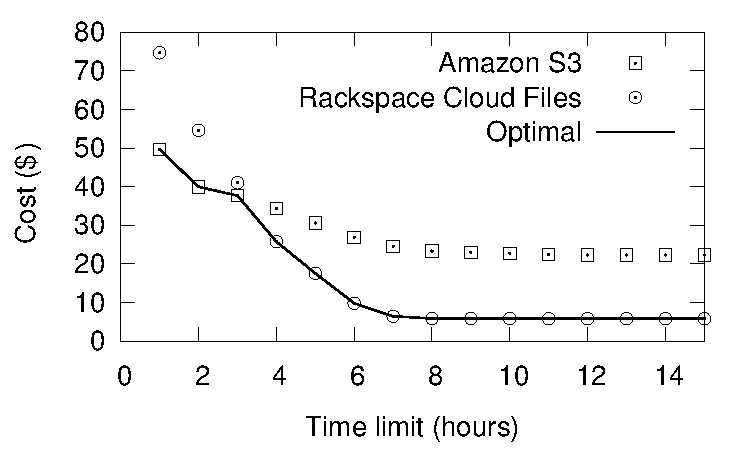
\includegraphics[width=\textwidth]{Workflow/Genome500-deadline_cost}
         \caption{500 tasks, 4 GiB data size}
         \label{fig:workflow:genome-500}
       \end{subfigure}
       \caption{\label{fig:workflow:genome}Result of the optimization procedure for the Epigenomics application.}
    \end{figure}  

    Fig.~\ref{fig:workflow:genome} shows the example results obtained for the Epigenomics application and workflows of two sizes (400 and 500 tasks). For longer deadlines the private cloud instances and the cheapest RackSpace instances are used so the cost is low when using CloudFiles. For shorter deadlines the cost grows rapidly, since we reach the limit of 15 instances per cloud and additional instances must be spawned on a different provider, making the transfer costs higher. This effect is amplified in Fig.~\ref{fig:workflow:genome-500}, which differs from Fig.~\ref{fig:workflow:genome-400} not only by the number of tasks but also by the data size of one layer. This means that the transfer costs are growing more rapidly, so it becomes more economical to store the data on Amazon EC2 that provides more powerful instances required for short deadlines.
    
    \begin{figure}[tb]
       \centering 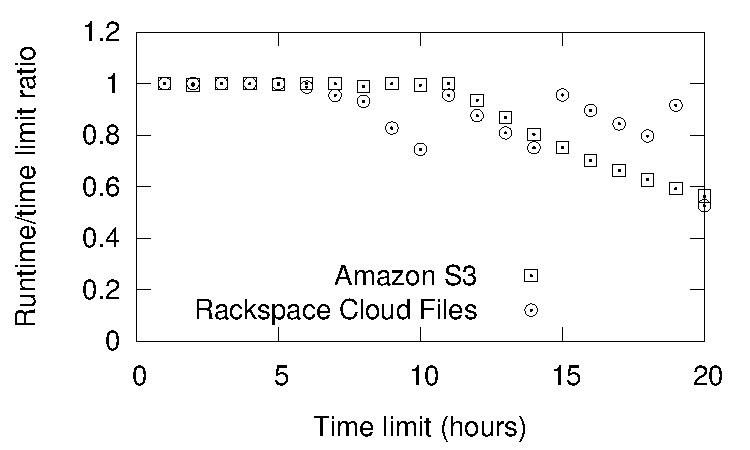
\includegraphics[width=0.7\textwidth]{Workflow/Genome500-time_ratio}
       \caption{Ratio of actual completion time to deadline for Epigenomics workflow with 500 tasks.
       \label{fig:workflow:genome-500-ratio}}
    \end{figure}
    
    One interesting feature of our model is that for longer deadlines it can find the cost-optimal solutions that have shorter workflow completion time than the requested deadline. This effect can be observed in Fig.~\ref{fig:workflow:genome-500-ratio} and is caused by the fact that for long deadlines the simple solution is to run the application on a set of the least expensive machines. 
    
    \begin{figure}[tb] 
       \centering       
       \begin{subfigure}[b]{0.45\textwidth}
         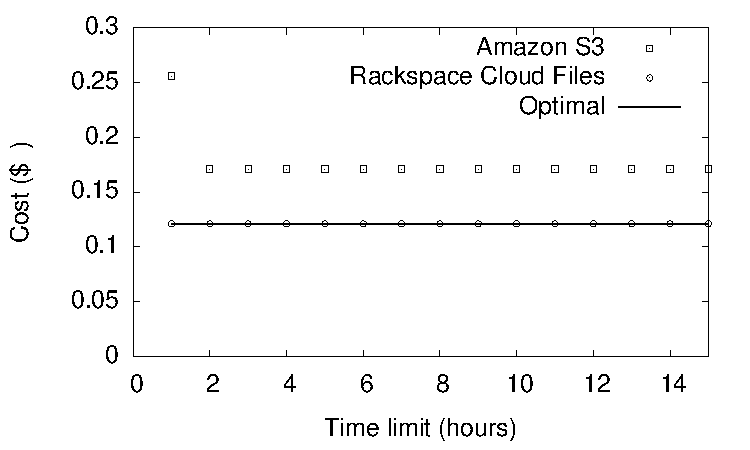
\includegraphics[width=\linewidth]{Workflow/CYBERSHAKE-100-deadline_cost}
         \caption{100 tasks}
       \end{subfigure}
       \begin{subfigure}[b]{0.45\textwidth}
         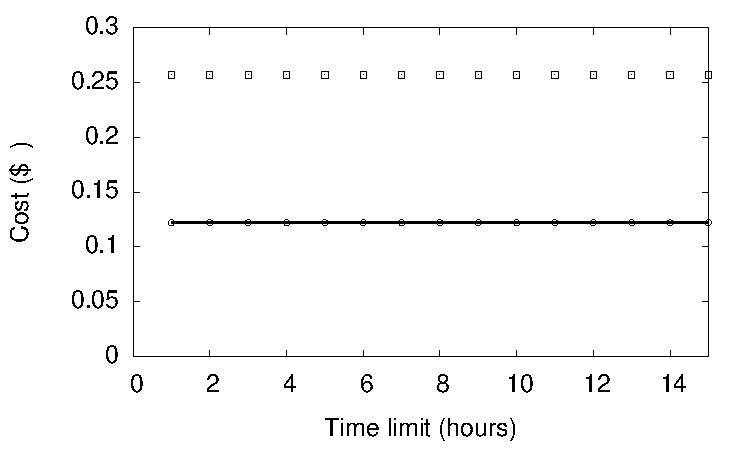
\includegraphics[width=\linewidth]{Workflow/CYBERSHAKE-200-deadline_cost}
         \caption{200 tasks}
       \end{subfigure}
       \begin{subfigure}[b]{0.45\textwidth}
         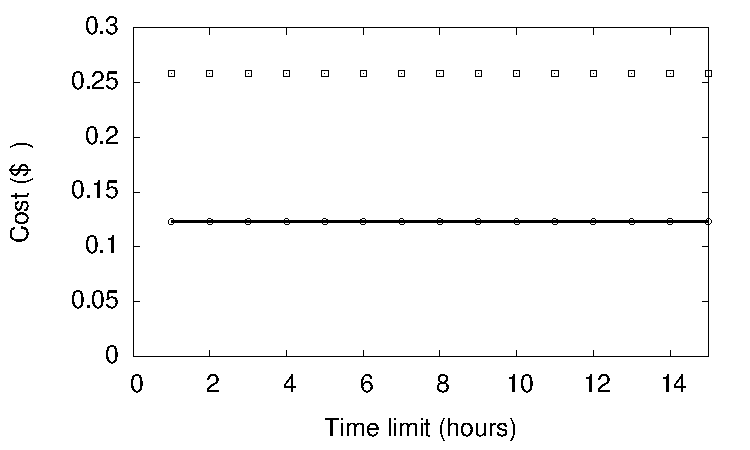
\includegraphics[width=\linewidth]{Workflow/CYBERSHAKE-300-deadline_cost}
         \caption{300 tasks}
       \end{subfigure}
       \begin{subfigure}[b]{0.45\textwidth}
         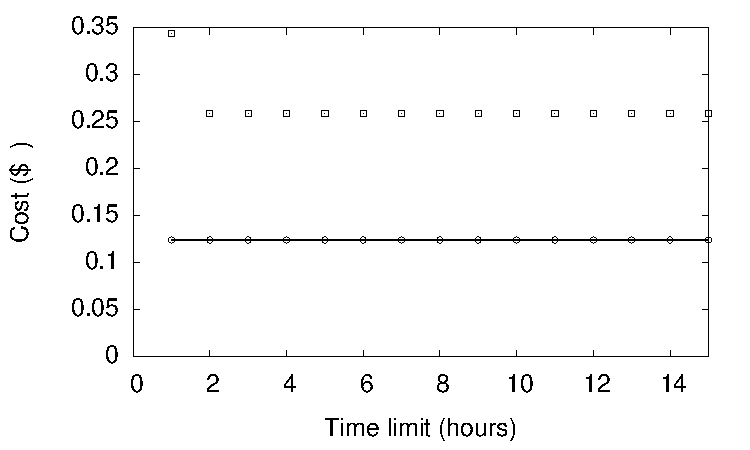
\includegraphics[width=\linewidth]{Workflow/CYBERSHAKE-400-deadline_cost}
         \caption{400 tasks}
       \end{subfigure}
       \begin{subfigure}[b]{0.45\textwidth}
         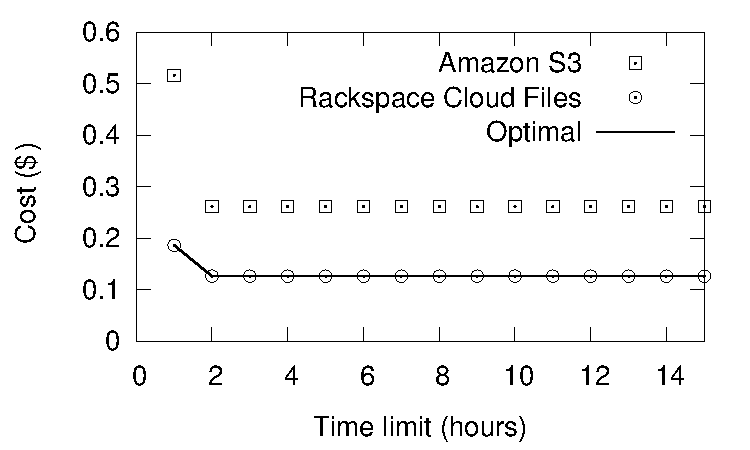
\includegraphics[width=\linewidth]{Workflow/CYBERSHAKE-500-deadline_cost}
         \caption{500 tasks}
       \end{subfigure}
       \begin{subfigure}[b]{0.45\textwidth}
         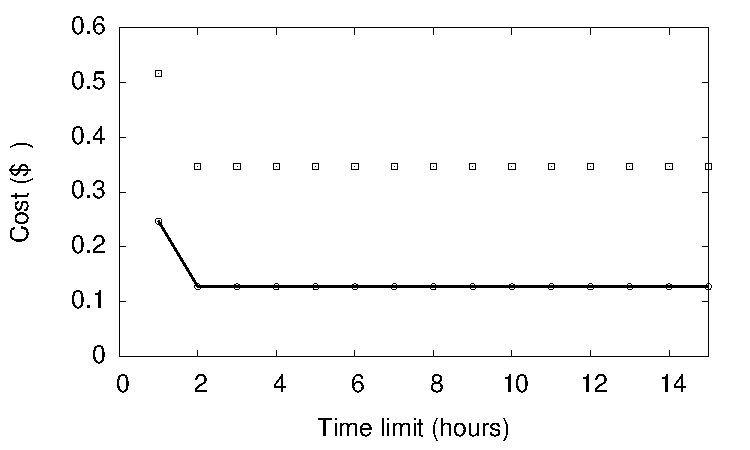
\includegraphics[width=\linewidth]{Workflow/CYBERSHAKE-700-deadline_cost}
         \caption{700 tasks}
       \end{subfigure}
       \begin{subfigure}[b]{0.45\textwidth}
         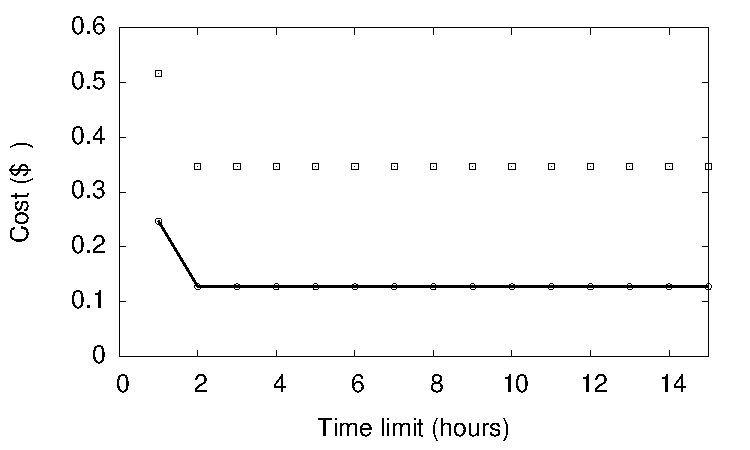
\includegraphics[width=\linewidth]{Workflow/CYBERSHAKE-600-deadline_cost}
         \caption{600 tasks}
       \end{subfigure}
       \begin{subfigure}[b]{0.45\textwidth}
         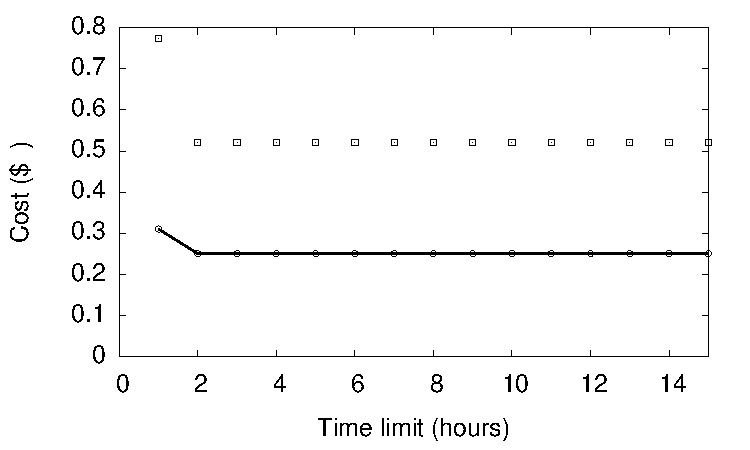
\includegraphics[width=\linewidth]{Workflow/CYBERSHAKE-900-deadline_cost}
         \caption{900 tasks}
       \end{subfigure}
       \begin{subfigure}[b]{0.45\textwidth}
         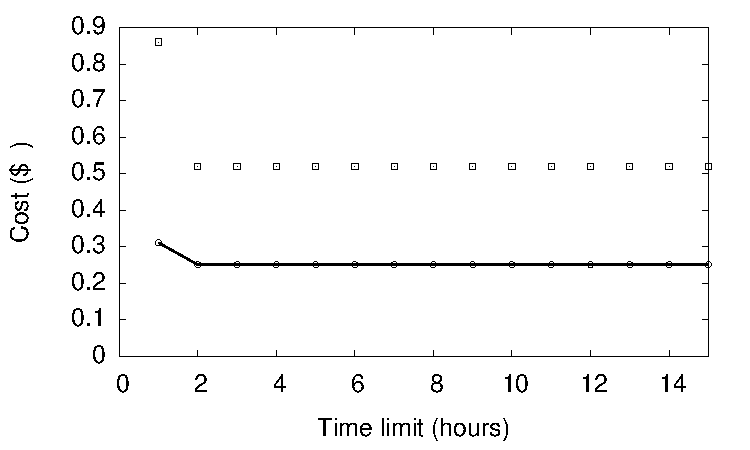
\includegraphics[width=\linewidth]{Workflow/CYBERSHAKE-1000-deadline_cost}
         \caption{1000 tasks}
       \end{subfigure}
       \caption{Optimal cost found by the model for CyberShake workflow.}
       \label{fig:workflow:cybershake}
     \end{figure}
     
     \begin{figure}[tb] 
       \centering       
       % \begin{subfigure}[b]{0.45\textwidth}
       %   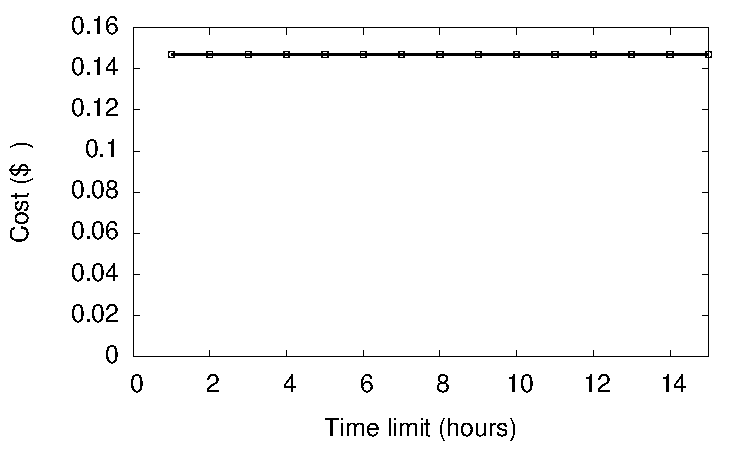
\includegraphics[width=\linewidth]{Workflow/LIGO-50-deadline_cost}
       %   \caption{50 tasks}
       % \end{subfigure}
       \begin{subfigure}[b]{0.45\textwidth}
         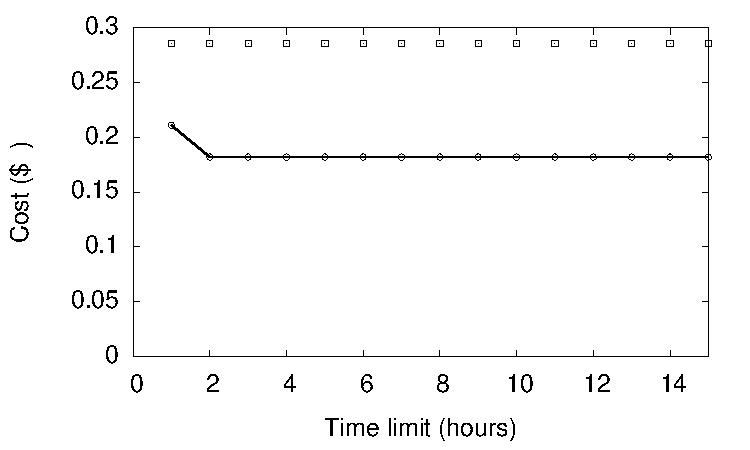
\includegraphics[width=\linewidth]{Workflow/LIGO-100-deadline_cost}
         \caption{100 tasks}
       \end{subfigure}
       \begin{subfigure}[b]{0.45\textwidth}
         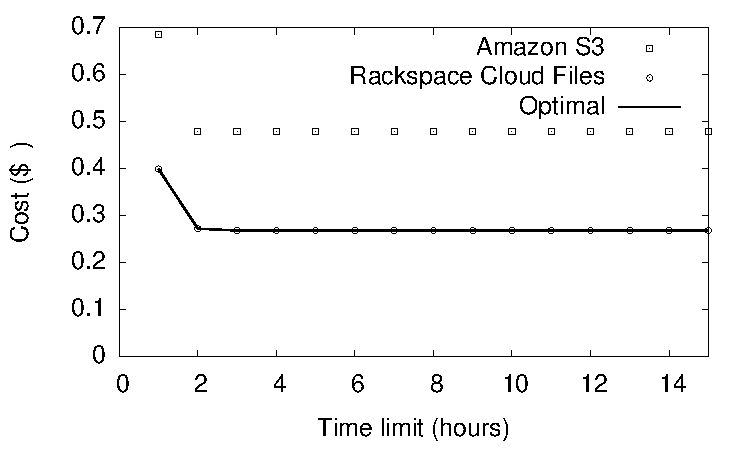
\includegraphics[width=\linewidth]{Workflow/LIGO-200-deadline_cost}
         \caption{200 tasks}
       \end{subfigure}
       \begin{subfigure}[b]{0.45\textwidth}
         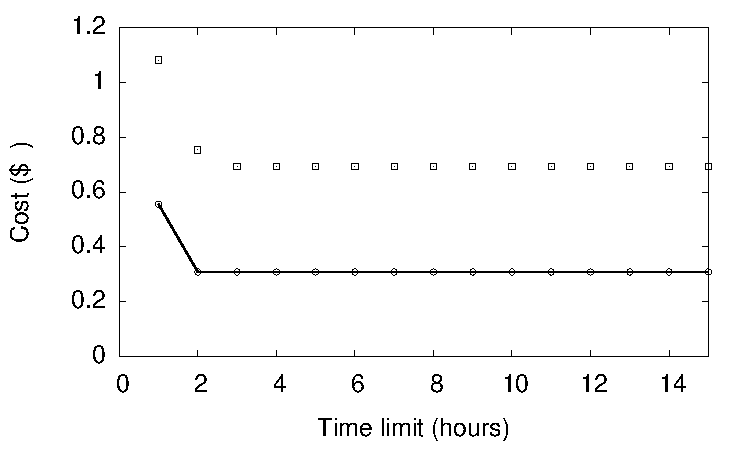
\includegraphics[width=\linewidth]{Workflow/LIGO-300-deadline_cost}
         \caption{300 tasks}
       \end{subfigure}
       \begin{subfigure}[b]{0.45\textwidth}
         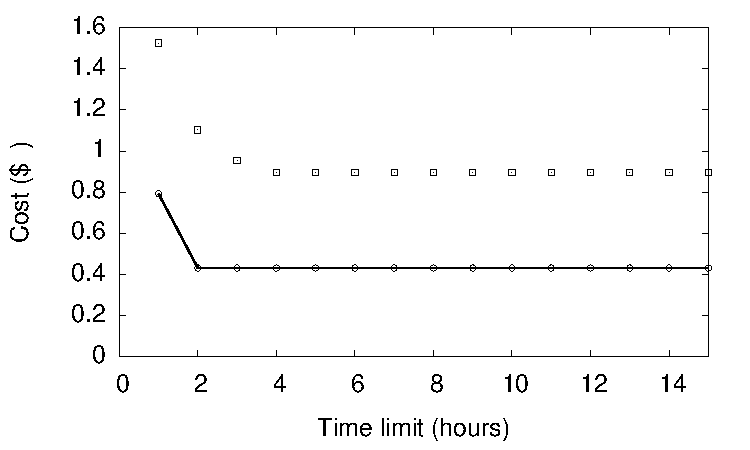
\includegraphics[width=\linewidth]{Workflow/LIGO-400-deadline_cost}
         \caption{400 tasks}
       \end{subfigure}
       \begin{subfigure}[b]{0.45\textwidth}
         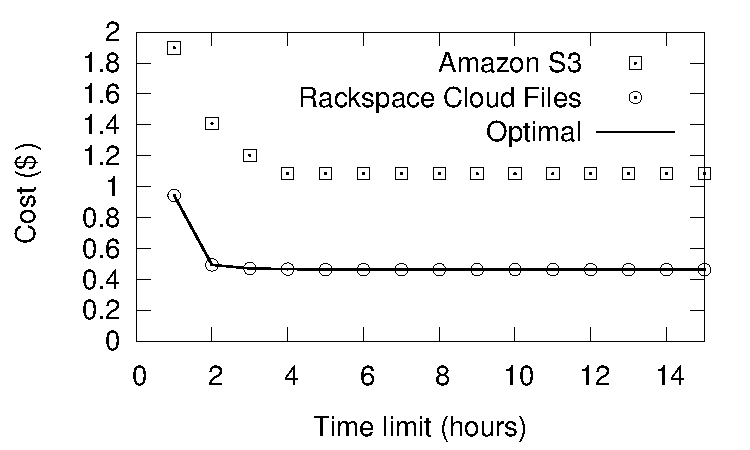
\includegraphics[width=\linewidth]{Workflow/LIGO-500-deadline_cost}
         \caption{500 tasks}
       \end{subfigure}
       \begin{subfigure}[b]{0.45\textwidth}
         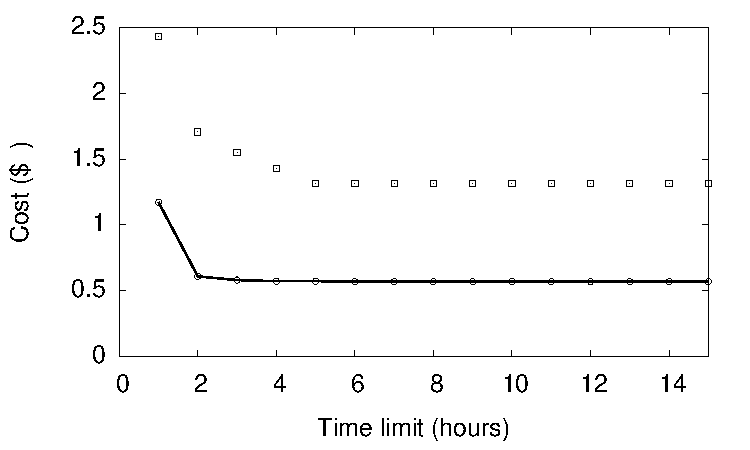
\includegraphics[width=\linewidth]{Workflow/LIGO-600-deadline_cost}
         \caption{600 tasks}
       \end{subfigure}
       \begin{subfigure}[b]{0.45\textwidth}
         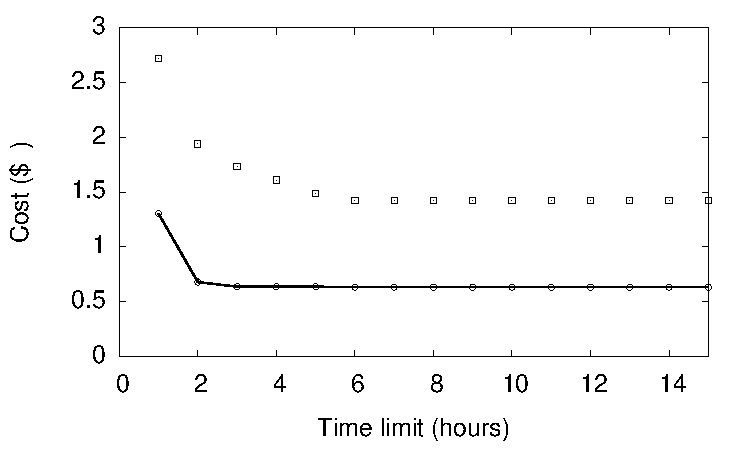
\includegraphics[width=\linewidth]{Workflow/LIGO-700-deadline_cost}
         \caption{700 tasks}
       \end{subfigure}
       \begin{subfigure}[b]{0.45\textwidth}
         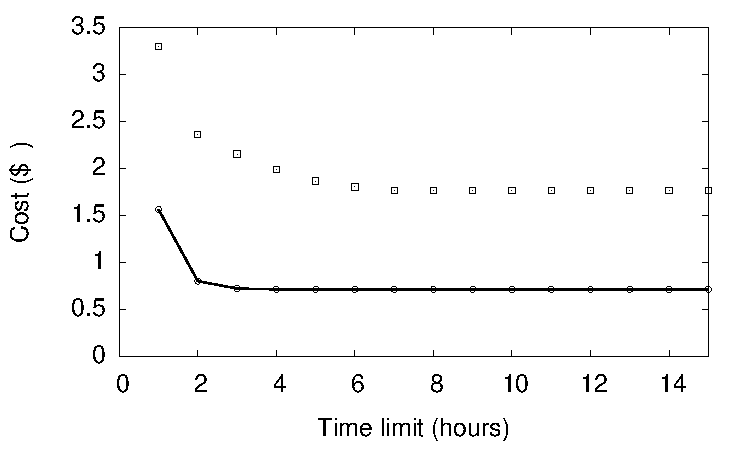
\includegraphics[width=\linewidth]{Workflow/LIGO-800-deadline_cost}
         \caption{800 tasks}
       \end{subfigure}
       \begin{subfigure}[b]{0.45\textwidth}
         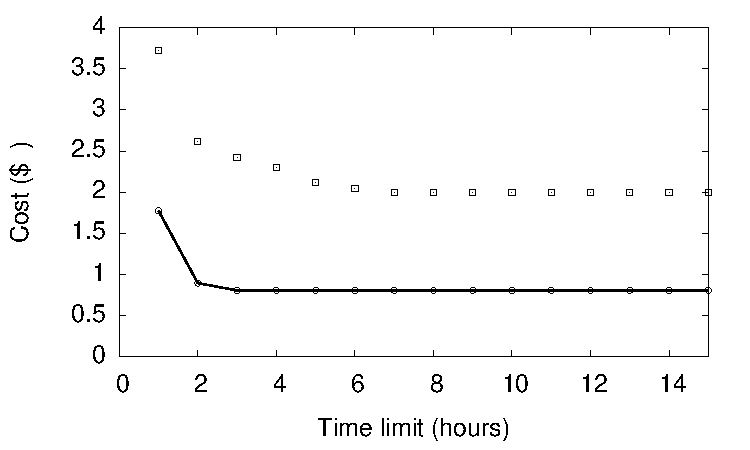
\includegraphics[width=\linewidth]{Workflow/LIGO-900-deadline_cost}
         \caption{900 tasks}
       \end{subfigure}
       \begin{subfigure}[b]{0.45\textwidth}
         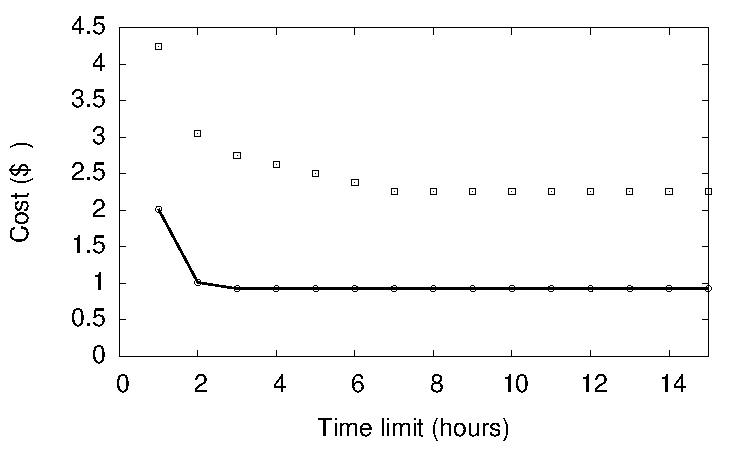
\includegraphics[width=\linewidth]{Workflow/LIGO-1000-deadline_cost}
         \caption{1000 tasks}
       \end{subfigure}
       \caption{Optimal cost found by the model for LIGO workflow.}
       \label{fig:workflow:ligo}
     \end{figure}
     
     \begin{figure}[tb] 
       \centering       
       \begin{subfigure}[b]{0.45\textwidth}
         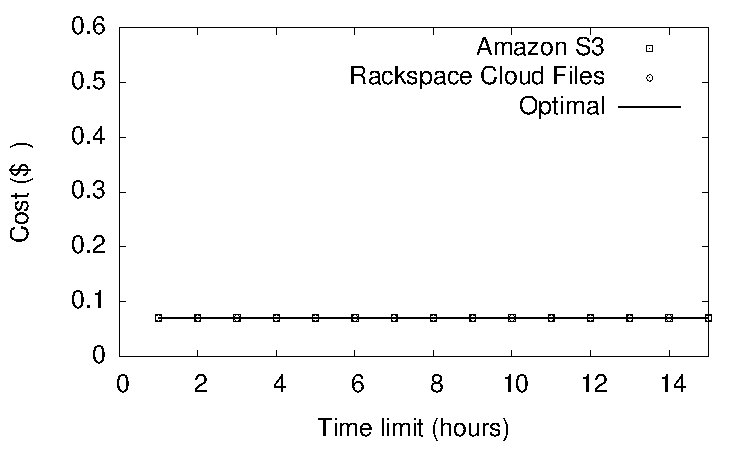
\includegraphics[width=\linewidth]{Workflow/MONTAGE-50-deadline_cost}
         \caption{50 tasks}
       \end{subfigure}
       \begin{subfigure}[b]{0.45\textwidth}
         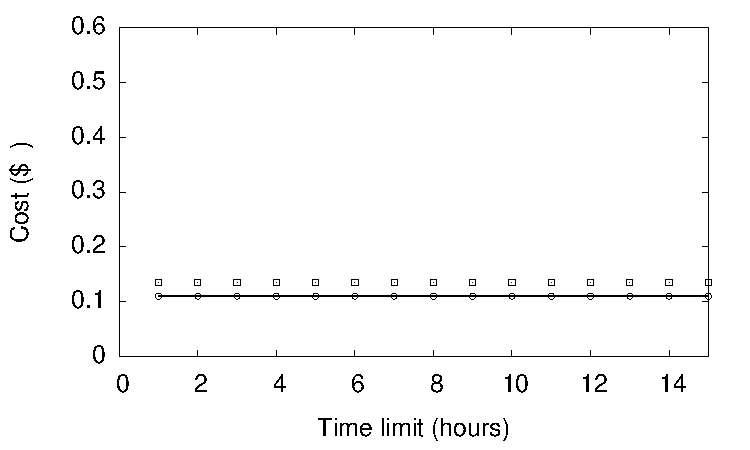
\includegraphics[width=\linewidth]{Workflow/MONTAGE-100-deadline_cost}
         \caption{100 tasks}
       \end{subfigure}
       \begin{subfigure}[b]{0.45\textwidth}
         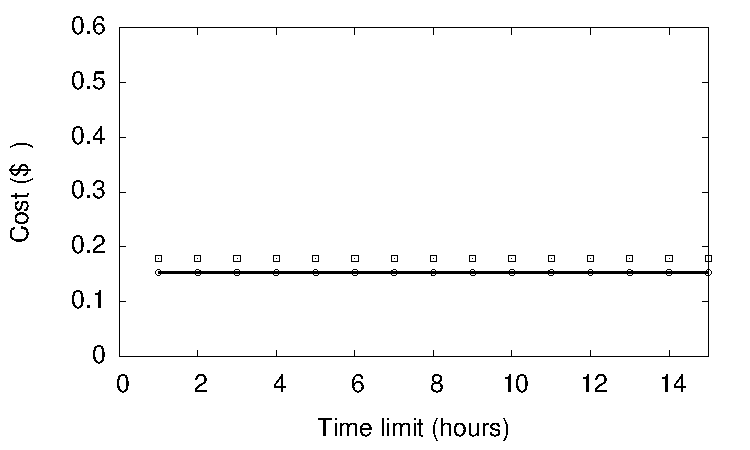
\includegraphics[width=\linewidth]{Workflow/MONTAGE-200-deadline_cost}
         \caption{200 tasks}
       \end{subfigure}
       \begin{subfigure}[b]{0.45\textwidth}
         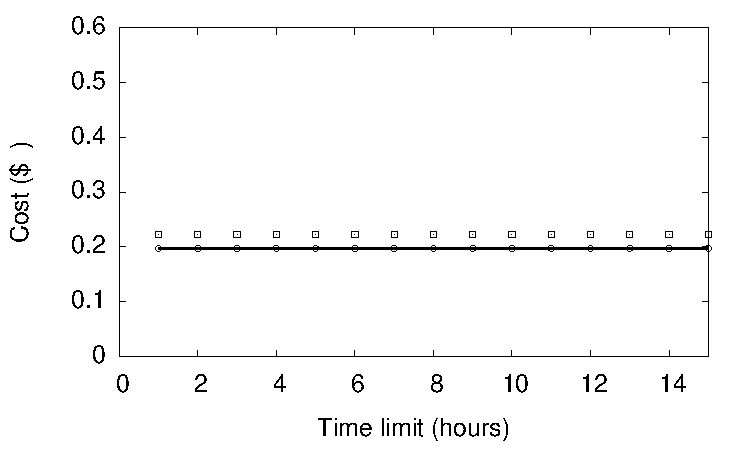
\includegraphics[width=\linewidth]{Workflow/MONTAGE-300-deadline_cost}
         \caption{300 tasks}
       \end{subfigure}
       \begin{subfigure}[b]{0.45\textwidth}
         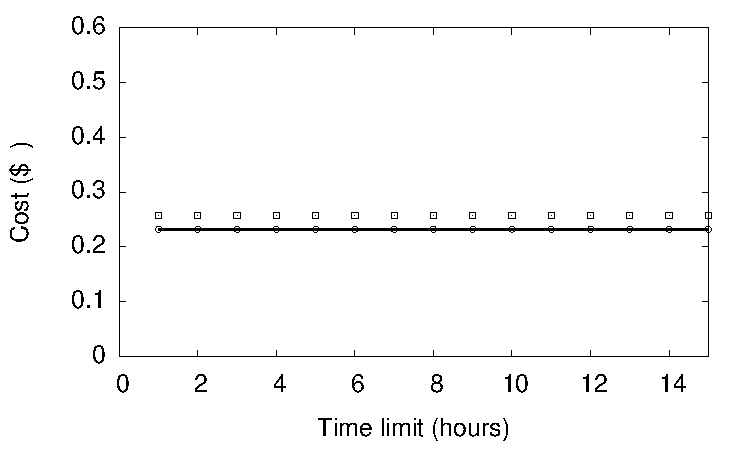
\includegraphics[width=\linewidth]{Workflow/MONTAGE-400-deadline_cost}
         \caption{400 tasks}
       \end{subfigure}
       \begin{subfigure}[b]{0.45\textwidth}
         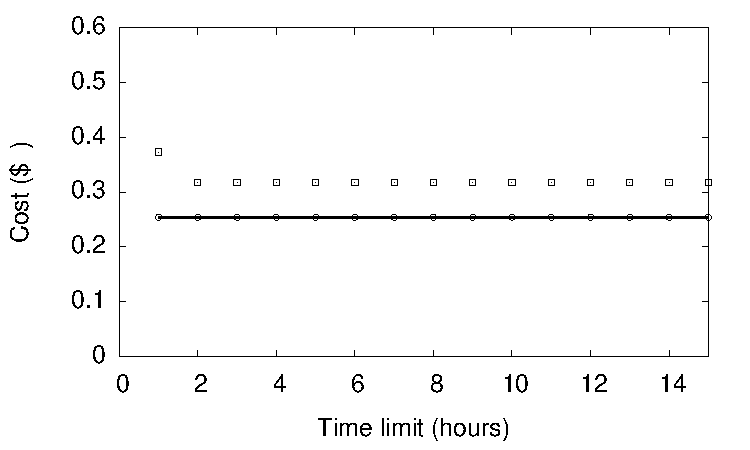
\includegraphics[width=\linewidth]{Workflow/MONTAGE-500-deadline_cost}
         \caption{\label{fig:workflow:montage-500}500 tasks}
       \end{subfigure}
       \begin{subfigure}[b]{0.45\textwidth}
         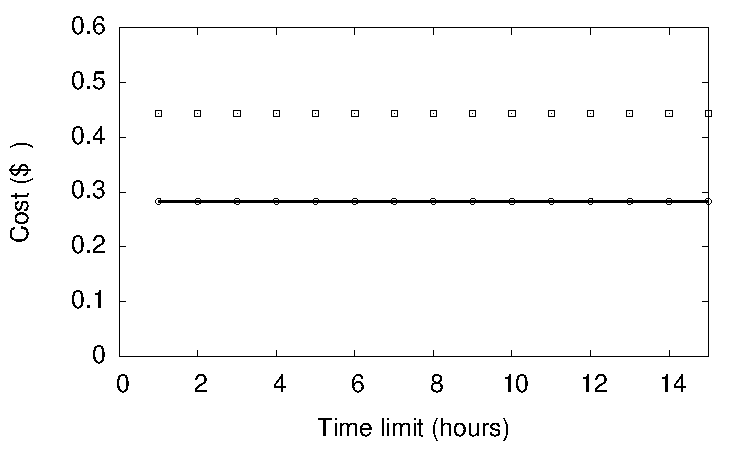
\includegraphics[width=\linewidth]{Workflow/MONTAGE-700-deadline_cost}
         \caption{700 tasks}
       \end{subfigure}
       \begin{subfigure}[b]{0.45\textwidth}
         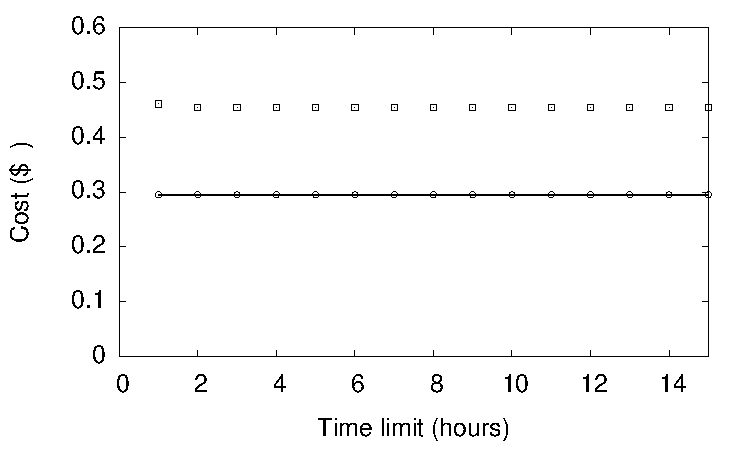
\includegraphics[width=\linewidth]{Workflow/MONTAGE-800-deadline_cost}
         \caption{800 tasks}
       \end{subfigure}
       \begin{subfigure}[b]{0.45\textwidth}
         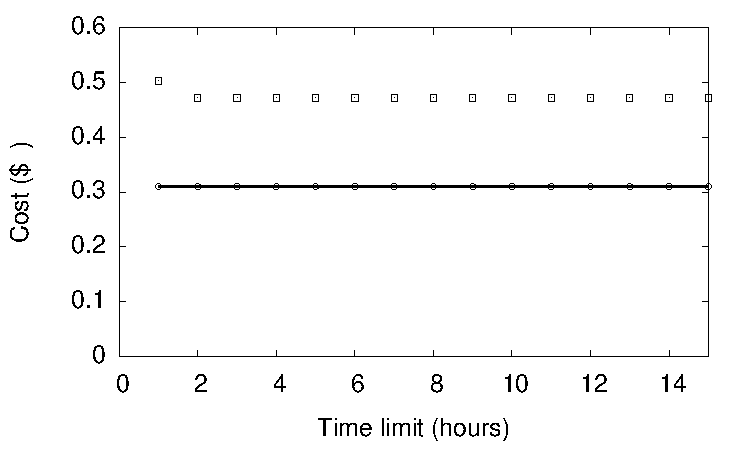
\includegraphics[width=\linewidth]{Workflow/MONTAGE-900-deadline_cost}
         \caption{900 tasks}
       \end{subfigure}
       \begin{subfigure}[b]{0.45\textwidth}
         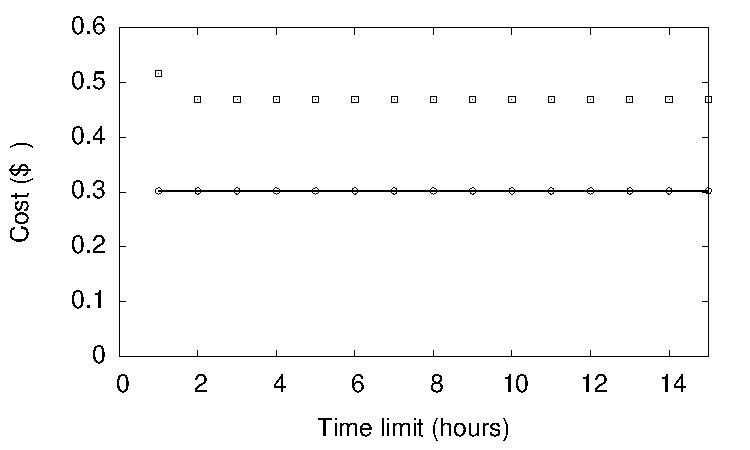
\includegraphics[width=\linewidth]{Workflow/MONTAGE-1000-deadline_cost}
         \caption{1000 tasks}
       \end{subfigure}
       \caption{Optimal cost found by the model for Montage workflow.}
       \label{fig:workflow:montage}
     \end{figure}
     
     \begin{figure}[tb] 
       \centering       
       \begin{subfigure}[b]{0.45\textwidth}
         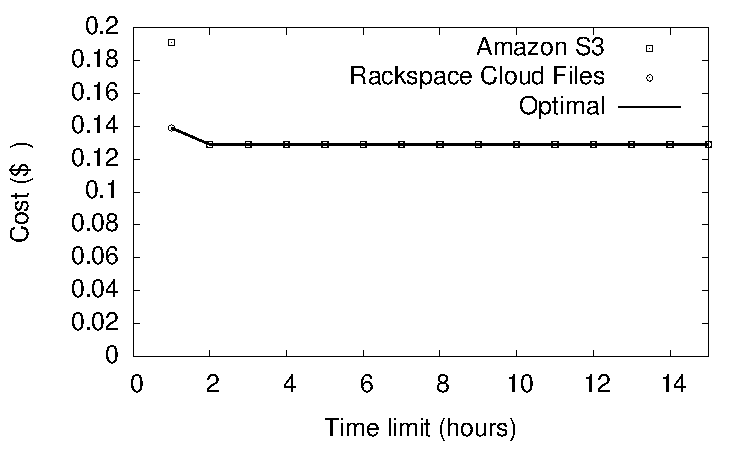
\includegraphics[width=\linewidth]{Workflow/SIPHT-50-deadline_cost}
         \caption{50 tasks}
       \end{subfigure}
       \begin{subfigure}[b]{0.45\textwidth}
         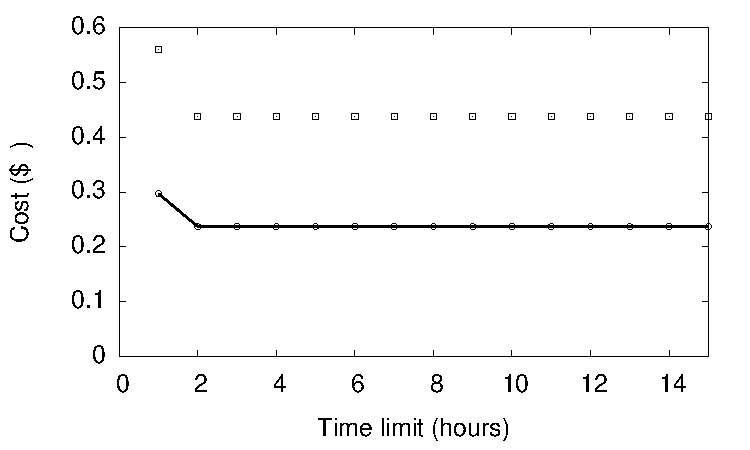
\includegraphics[width=\linewidth]{Workflow/SIPHT-200-deadline_cost}
         \caption{200 tasks}
       \end{subfigure}
       \begin{subfigure}[b]{0.45\textwidth}
         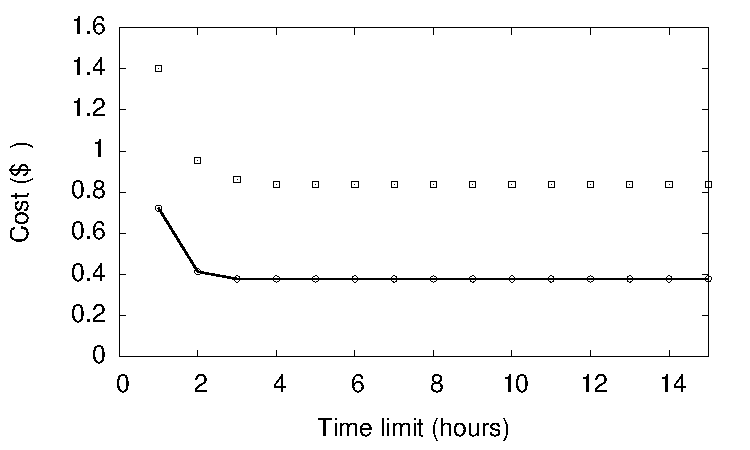
\includegraphics[width=\linewidth]{Workflow/SIPHT-400-deadline_cost}
         \caption{400 tasks}
       \end{subfigure}
       \begin{subfigure}[b]{0.45\textwidth}
         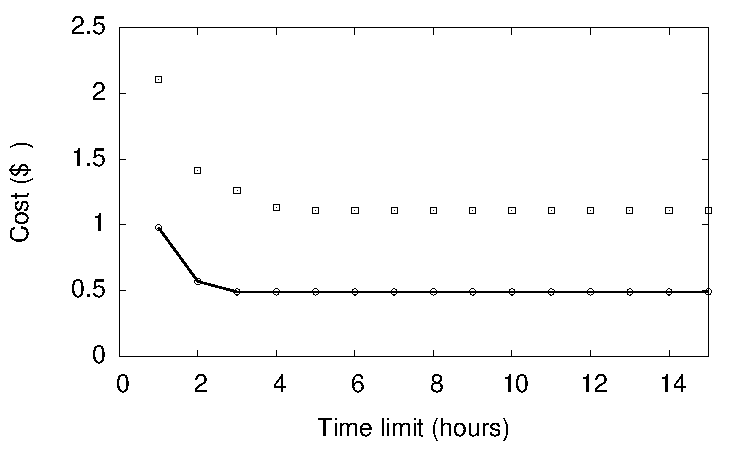
\includegraphics[width=\linewidth]{Workflow/SIPHT-600-deadline_cost}
         \caption{600 tasks}
       \end{subfigure}
       \begin{subfigure}[b]{0.45\textwidth}
         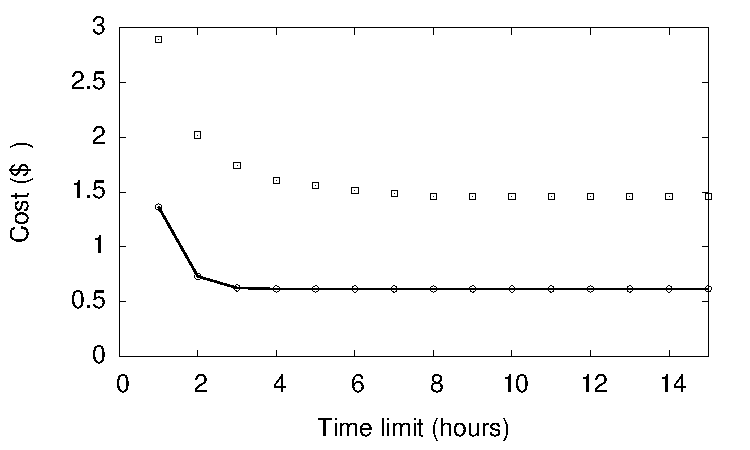
\includegraphics[width=\linewidth]{Workflow/SIPHT-800-deadline_cost}
         \caption{800 tasks}
       \end{subfigure}
       \begin{subfigure}[b]{0.45\textwidth}
         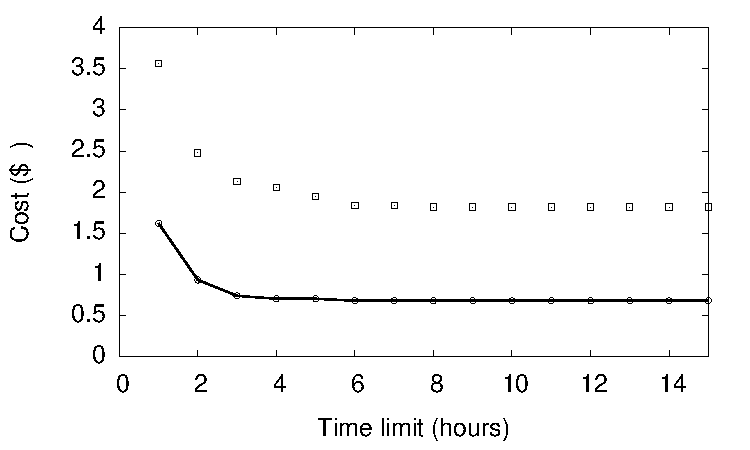
\includegraphics[width=\linewidth]{Workflow/SIPHT-1000-deadline_cost}
         \caption{1000 tasks}
       \end{subfigure}
       \begin{subfigure}[b]{0.45\textwidth}
         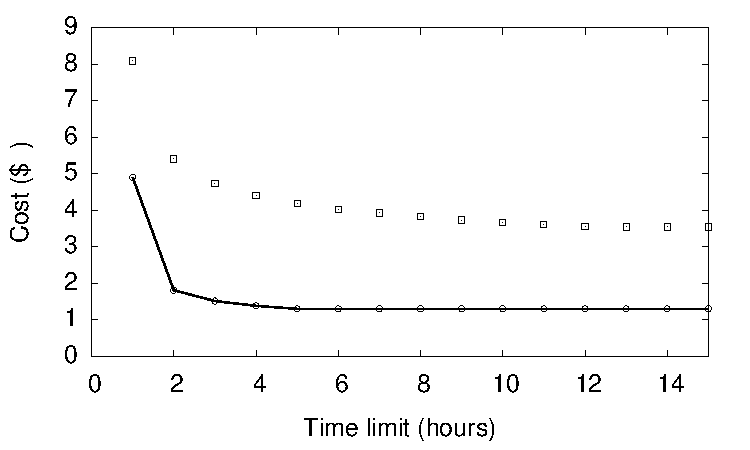
\includegraphics[width=\linewidth]{Workflow/SIPHT-2000-deadline_cost}
         \caption{2000 tasks}
       \end{subfigure}
       \begin{subfigure}[b]{0.45\textwidth}
         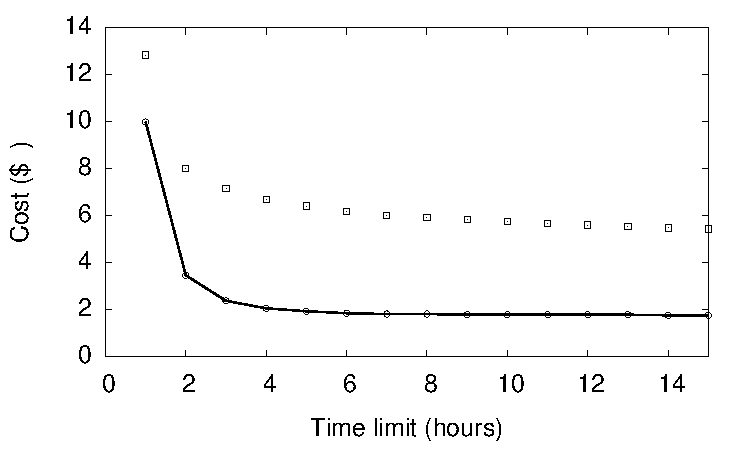
\includegraphics[width=\linewidth]{Workflow/SIPHT-3000-deadline_cost}
         \caption{3000 tasks}
       \end{subfigure}
       \begin{subfigure}[b]{0.45\textwidth}
         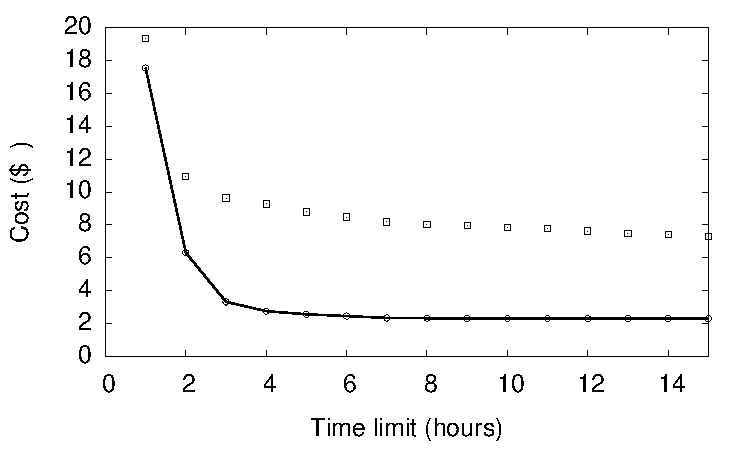
\includegraphics[width=\linewidth]{Workflow/SIPHT-4000-deadline_cost}
         \caption{4000 tasks}
       \end{subfigure}
       \begin{subfigure}[b]{0.45\textwidth}
         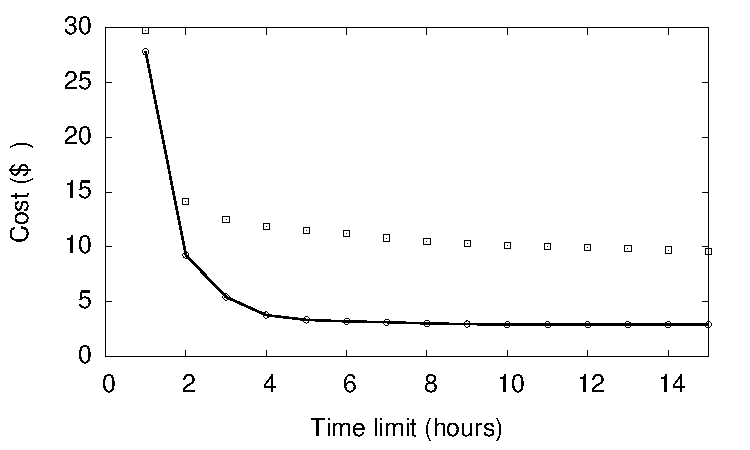
\includegraphics[width=\linewidth]{Workflow/SIPHT-5000-deadline_cost}
         \caption{5000 tasks}
       \end{subfigure}
       \caption{Optimal cost found by the model for SIPHT workflow.}
       \label{fig:workflow:sipht}
     \end{figure}
 
    Figures \ref{fig:workflow:cybershake} to \ref{fig:workflow:sipht} show results obtained for other workflows. These workflows are relatively small and even for short deadlines our model is able to schedule tasks to be executed in a very short time on cheapest instances on a single cloud, this results in flat characteristics.
    
    To investigate how the model behaves for workflows with the same structure, but with much longer run times of tasks, we run the optimization for Montage workflow with tasks $1000 \times$ longer. This corresponds to the scenario where tasks are in the order of hours instead of seconds. The sample results in Fig.~\ref{fig:workflow:montage-500x1000} show how the cost increases much steeply with shorter deadlines, illustrating the trade-off between time and cost. The difference between Figs.~\ref{fig:workflow:montage-500}~and~\ref{fig:workflow:montage-500x1000} illustrates that the model is more useful for workflows when tasks are of granularity that is similar to the granularity of the (hourly) billing cycle of cloud providers.    

    \begin{figure}[tb]
       \centering 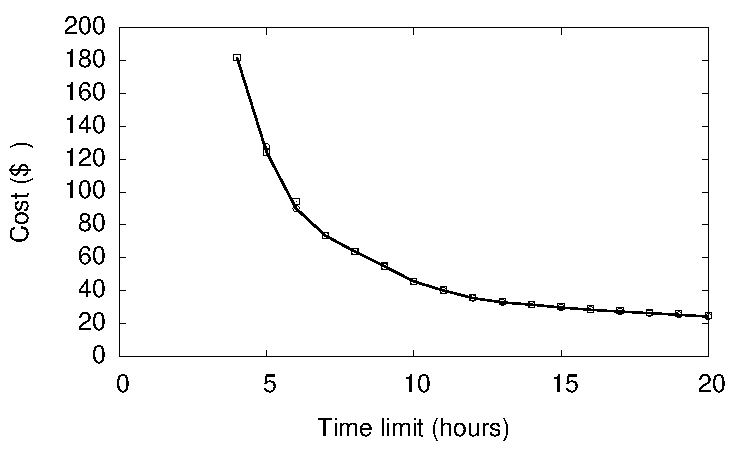
\includegraphics[width=0.7\textwidth]{Workflow/MONTAGE-500x1000-deadline_cost}
       \caption{Optimal cost obtained by the model for Montage 500 workflow with tasks runtimes artificailly 
       multiplied by 1000.
       \label{fig:workflow:montage-500x1000}}
    \end{figure}

    \begin{figure}[tb] 
       \centering
       
       \begin{subfigure}[b]{0.7\textwidth}  
         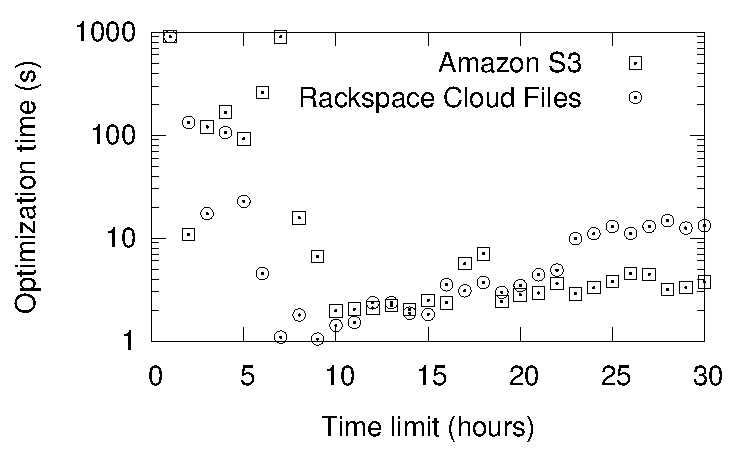
\includegraphics[width=\linewidth]{Workflow/Genome600-wall_time}
         \caption{Epigenomics, 600 tasks}
         \label{fig:workflow:genome-600-opttime}
       \end{subfigure}
       \begin{subfigure}[b]{0.7\textwidth}
         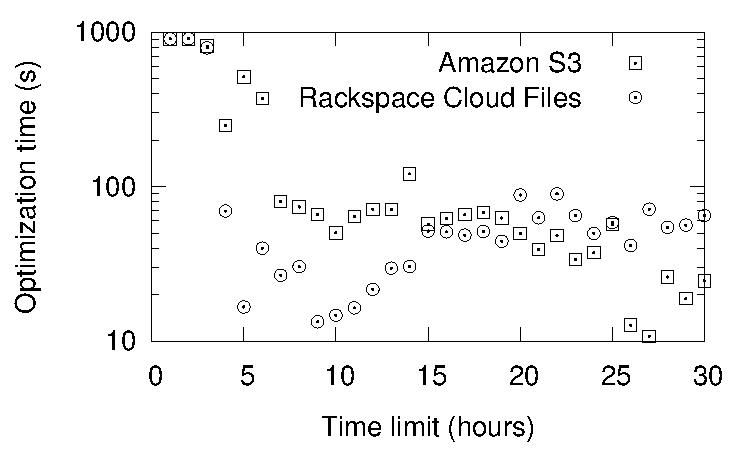
\includegraphics[width=\linewidth]{Workflow/SIPHT-5000-wall_time}
         \caption{SIPHT, 5000 tasks}
         \label{fig:workflow:sipht-5000-opttime}
       \end{subfigure}
       
       \caption{Solver execution wall time.}
    \end{figure}
  
    
    The run time of the optimization algorithm for workflows with up to 1000 tasks ranges from few seconds up to 4 minutes using the CPLEX~\cite{cplex} solver running on a server with 4 16-core 2.3 GHz AMD Opteron processors (model 6276), with a limit set to 32 cores. Fig.~\ref{fig:workflow:genome-600-opttime} shows that the time becomes much higher for shorter deadlines and increases for very long deadlines. This is correlated with size of search space: the longer the deadline, the search space is larger, while for shorter deadlines the problem has a very small set of acceptable solutions.  The problem becomes more severe for bigger and more complex workflows like SIPHT as optimization time becomes very high (Fig.~\ref{fig:workflow:sipht-5000-opttime}).
    
\section{Summary}

    In this chapter, we presented a cost optimization model for scientific workflows executing on multiple heterogeneous clouds. The model, formulated in AMPL, allows us to find the optimal assignment of workflow tasks, grouped into layers, to cloud instances. The model was tested on a set of benchmark workflows and we observed that it gives useful solutions in a reasonable amount of computing time.  By solving the model for multiple deadlines, we can produce trade-off plots, showing how the cost depends on the deadline. Such plots are a step towards a scientific cloud workflow calculator, supporting resource management decisions for both end-users and workflow-as-a-service providers.
  
} % Command scope